\documentclass[11pt]{article}

\usepackage{classDM17}
\usepackage{hyperref}
\usepackage{float}
\usepackage{amsmath}
\newcommand{\D}{\textsf{D}}
\newcommand{\BigO}[1]{\mathcal{O}\left( #1 \right)}

\title{Assignmentmt 3: Clustering}
\author{Christopher Mertin/\verb~u1010077~\\\url{cmertin@cs.utah.edu}}
\date{\today}

\begin{document}
\maketitle




%%%%%%%%%%%%%%%%%%%%%%%%%%%%%%%%%%%%%%%%%%%%%%%%%%%%
%%%%%%%%%%%%%%%%%%%%%%%%%%%%%%%%%%%%%%%%%%%%%%%%%%%%
%%%%%%%%%%%%%%%%%%%%%%%%%%%%%%%%%%%%%%%%%%%%%%%%%%%%
\section*{Overview}

In this assignment you will explore clustering: hierarchical and point-assignment.  
You will also experiment with high dimensional data.  

You will use three data sets for this assignment:
\begin{itemize} \denselist
\item \href{http://www.cs.utah.edu/~jeffp/teaching/cs5140/A3/C1.txt}{\texttt{http://www.cs.utah.edu/\~{}jeffp/teaching/cs5140/A3/C1.txt}}
\item \href{http://www.cs.utah.edu/~jeffp/teaching/cs5140/A3/C2.txt}{\texttt{http://www.cs.utah.edu/\~{}jeffp/teaching/cs5140/A3/C2.txt}}
\item \href{http://www.cs.utah.edu/~jeffp/teaching/cs5140/A3/C3.txt}{\texttt{http://www.cs.utah.edu/\~{}jeffp/teaching/cs5140/A3/C3.txt}}
\end{itemize}
These data sets all have the following format.  Each line is a data point.  The lines have either 3 or 6 tab separated items.  The first one is an integer describing the index of the points.  The next 2 (or 5 for \texttt{C3}) are the coordinates of the data point.  \texttt{C1} and \texttt{C2} are in 2 dimensions, and \texttt{C3} is in 5 dimensions.  \texttt{C1} should have $n$=20 points, \texttt{C2} should have $n$=1004 points, and \texttt{C3} should have $n$=1000 points.  
We will always measure distance with Euclidean distance.  


\vspace{.1in}

\emph{As usual, it is highly recommended that you use LaTeX for this assignment.  If you do not, you may lose points if your assignment is difficult to read or hard to follow.  Find a sample form in this directory:
\url{http://www.cs.utah.edu/~jeffp/teaching/latex/}}


%%%%%%%%%%%%%%%%%%%%%%%%%%%%%%%%%%%%%%%%%%%%%%%%%%%%
%%%%%%%%%%%%%%%%%%%%%%%%%%%%%%%%%%%%%%%%%%%%%%%%%%%%
%%%%%%%%%%%%%%%%%%%%%%%%%%%%%%%%%%%%%%%%%%%%%%%%%%%%
\section{Hierarchical Clustering (20 points)}

There are many variants of hierarchical clustering; here we explore $3$.  The key difference is how you measure the distance $d(S_1, S_2)$ between two clusters $S_1$ and $S_2$.  
\begin{itemize}
\item[\textsf{Single-Link: }] measures the shortest link $\displaystyle{d(S_1,S_2) = \min_{(s_1,s_2) \in S_1 \times S_2} \|s_1 - s_2\|_2}$. 

\item[\textsf{Complete-Link: }] measures the longest link $\displaystyle{d(S_1,S_2) = \max_{(s_1,s_2) \in S_1 \times S_2} \|s_1 - s_2\|_2}$. 

\item[\textsf{Mean-Link: }] measures the distances to the means.  First compute 
$a_1 = \frac{1}{|S_1|} \sum_{s \in S_1} s$ and 
$a_2 = \frac{1}{|S_2|} \sum_{s \in S_2} s$ then
$\displaystyle{d(S_1, S_2) = \|a_1 - a_2\|_2}$ .
\end{itemize}

\paragraph{A (20 points):}  
Run all hierarchical clustering variants on data set \texttt{C1.txt} until there are $k=4$ clusters, and report the results as sets.  
It may be useful to do this pictorially.  

Which variant did the best job, and which was the easiest to compute (think if the data was much larger)?  
Explain your answers.  

\begin{figure}[H]
\centering
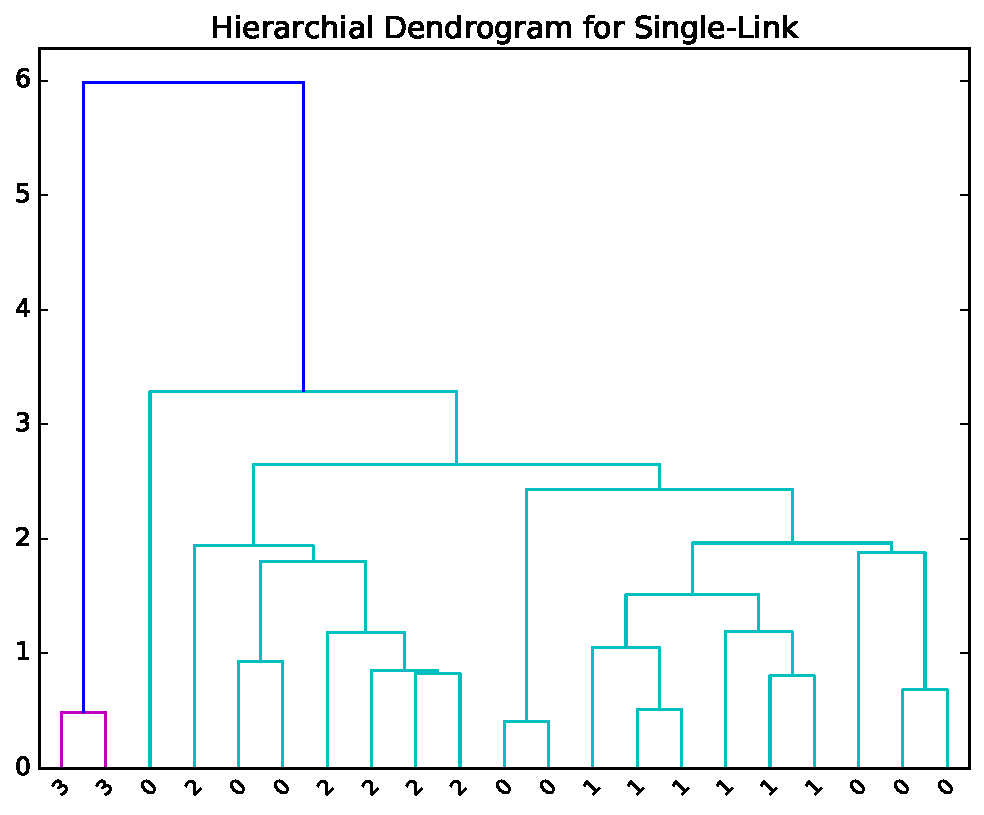
\includegraphics[width=.75\textwidth]{Single-Link_dendro.pdf}
\caption{Dendrogram for single link}
\end{figure}

\begin{figure}[H]
\centering
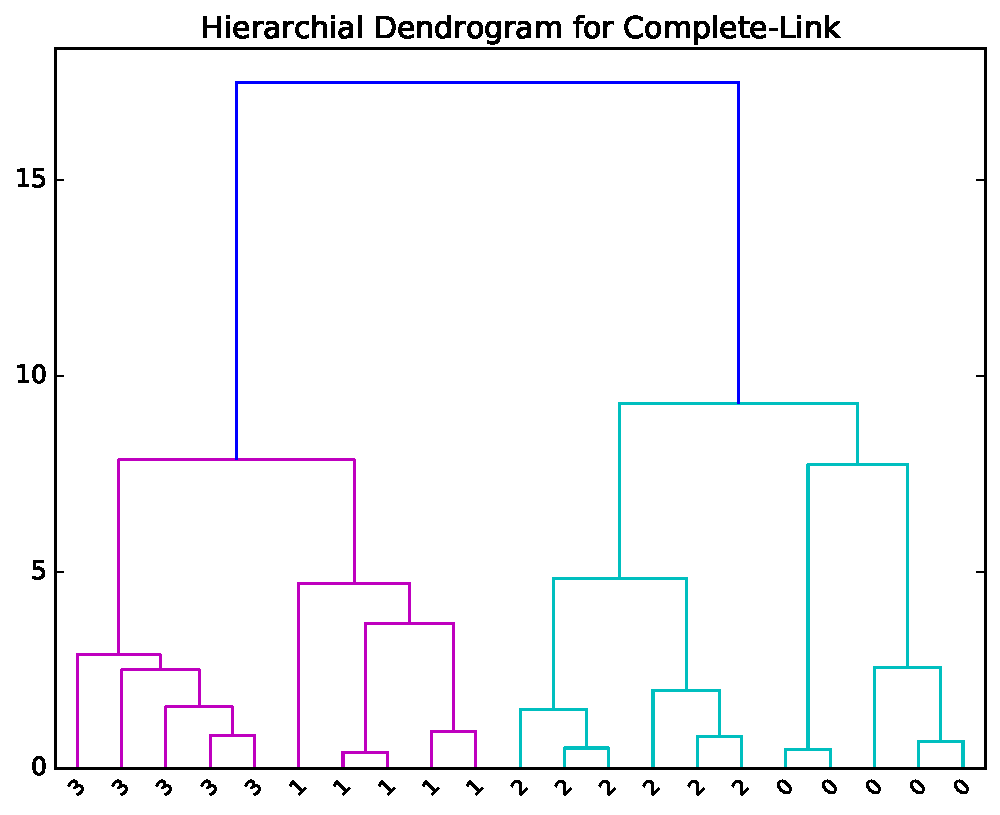
\includegraphics[width=.75\textwidth]{Complete-Link_dendro.pdf}
\caption{Dendrogram for complete link}
\end{figure}

\begin{figure}[H]
\centering
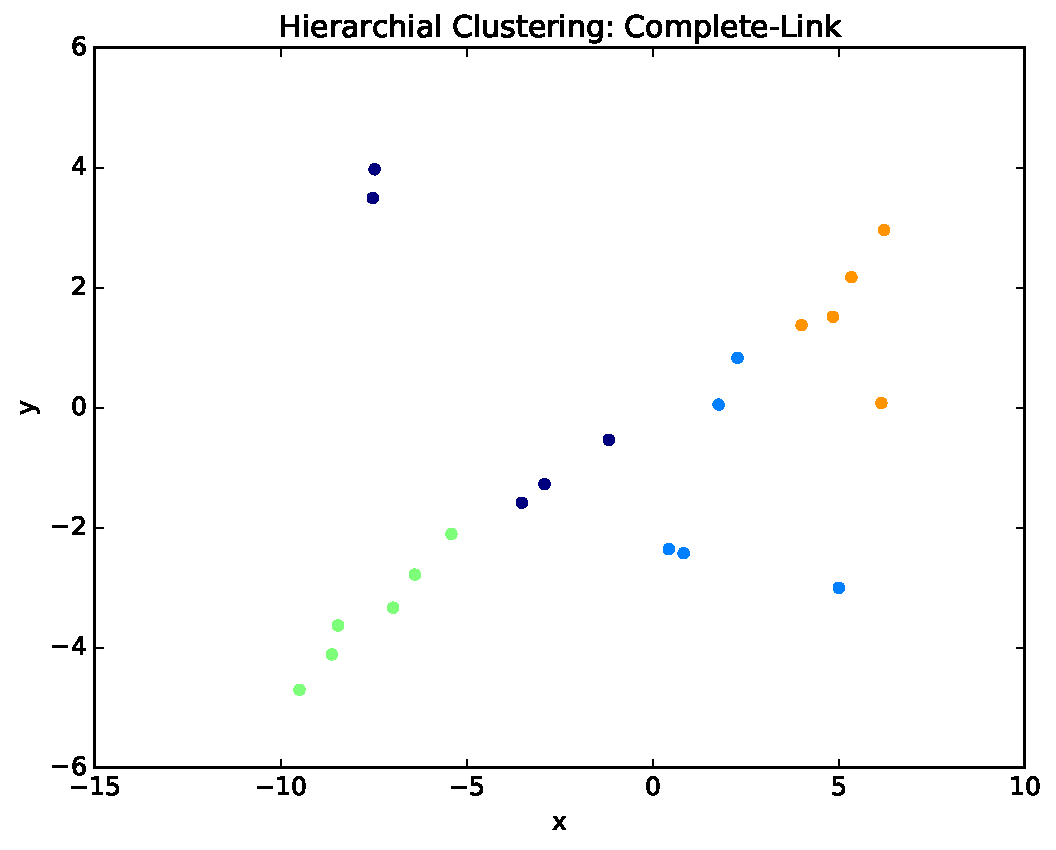
\includegraphics[width=.75\textwidth]{Complete-Link.pdf}
\caption{Clustering of points with Complete-Link}
\end{figure}

\begin{figure}[H]
\centering
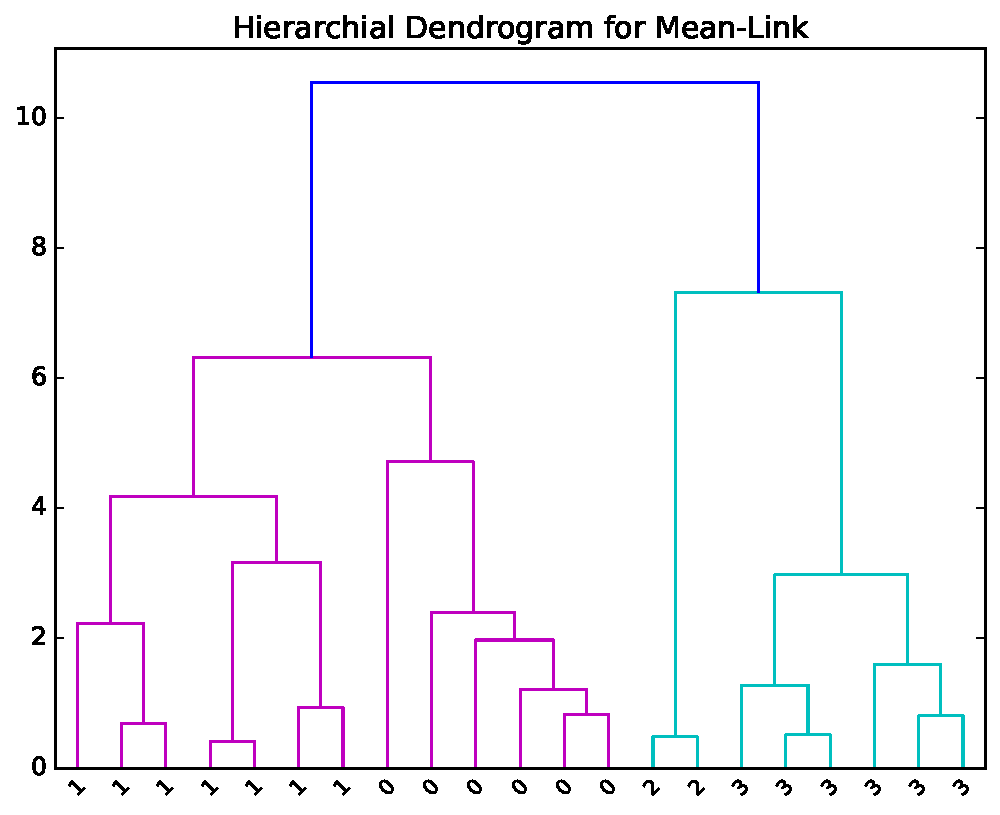
\includegraphics[width=.75\textwidth]{Mean-Link_dendro.pdf}
\caption{Dendrogram for Mean-Link}
\end{figure}

\begin{figure}[H]
\centering
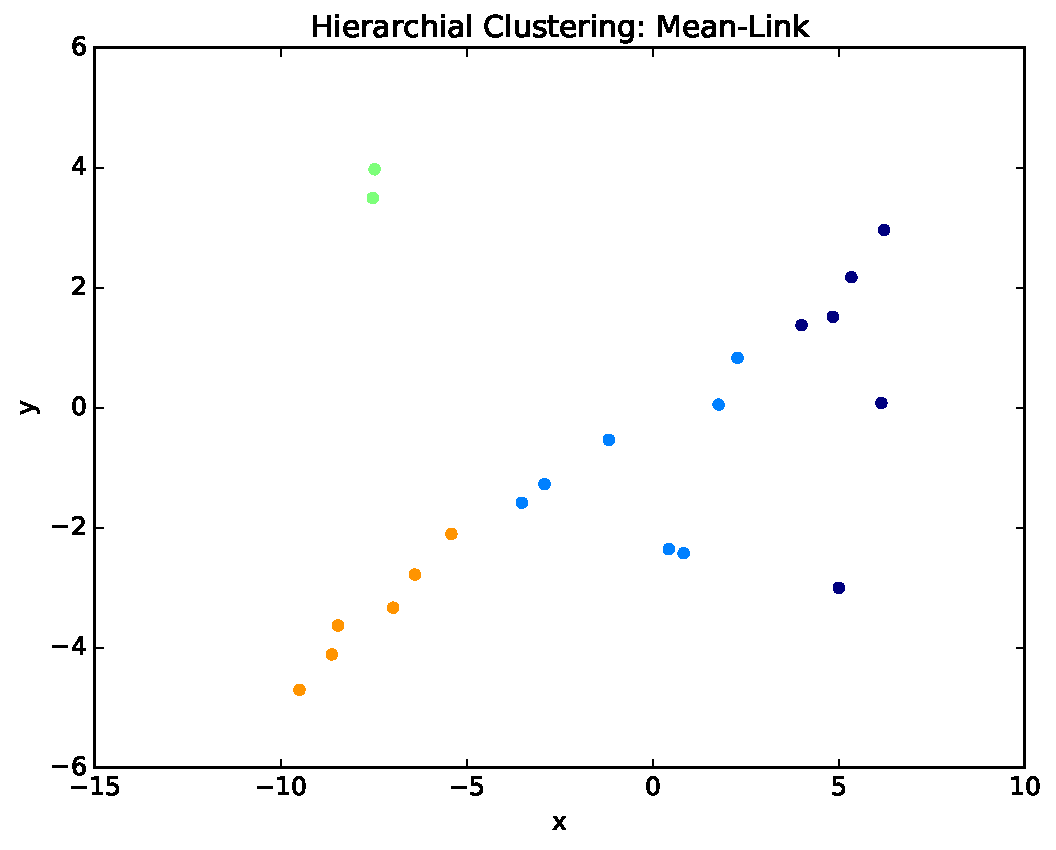
\includegraphics[width=.75\textwidth]{Mean-Link.pdf}
\caption{Clustering of points with Mean-Link}
\end{figure}



%%%%%%%%%%%%%%%%%%%%%%%%%%%%%%%%%%%%%%%%%%%%%%%%%%%%
%%%%%%%%%%%%%%%%%%%%%%%%%%%%%%%%%%%%%%%%%%%%%%%%%%%%
%%%%%%%%%%%%%%%%%%%%%%%%%%%%%%%%%%%%%%%%%%%%%%%%%%%%
\section{Assignment-Based Clustering (40 points)}

Assignment-based clustering works by assigning every point $x \in X$ to the closest cluster centers $C$.  Let $\phi_C : X \to C$ be this assignment map so that 
$\phi_C(x) = \arg \min_{c \in C} \D(x,c)$.  All points that map to the same cluster center are in the same cluster.  

Two good heuristics for these types of cluster are the 
\textsf{Gonzalez} (Algorithm 9.4.1) and \textsf{$k$-Means++} (Algorithm 10.1.2) algorithms.  

\paragraph{A: (20 points)}
Run \textsf{Gonzalez} and \textsf{k-Means++} on data set \texttt{C2.txt} for $k=3$. 
To avoid too much variation in the results, choose $c_1$ as the point with index \texttt{1}.  

Report the centers and the subsets (as pictures) for \textsf{Gonzalez}.  Report:
\begin{itemize} \denselist
\item the $3$-center cost $\max_{x \in X} \D(x,\phi_C(x))$  and 
\item the $3$-means cost $\sqrt{\frac{1}{|X|}\sum_{x \in X} (\D(x,\phi_C(x)))^2}$
  \\ (Note this has been normalized so easy to compare to $3$-center cost)
\end{itemize}


For \textsf{k-Means++}, the algorithm is randomized, so you will need to report the variation in this algorithm.  Run it several trials (at least $20$) and plot the \emph{cumulative density function} of the $3$-means cost.  
Also report what fraction of the time the subsets are the same as the result from \textsf{Gonzalez}.  

\begin{figure}[H]
\centering
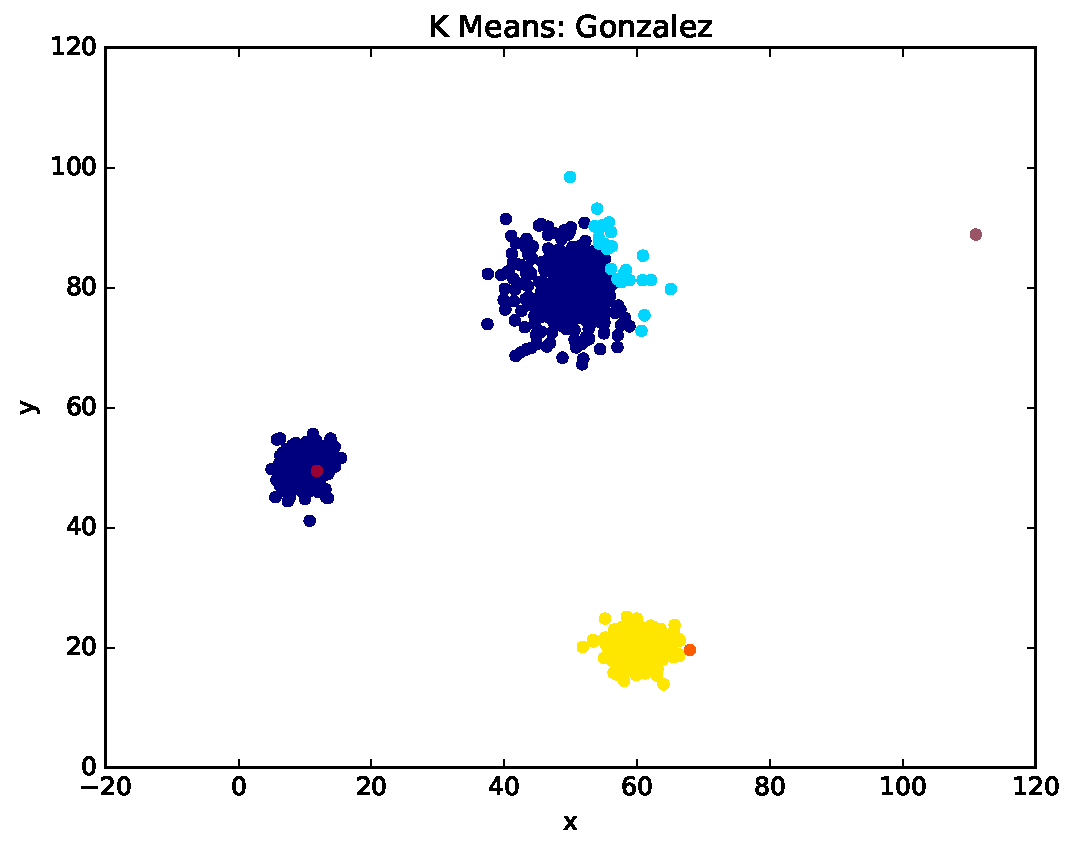
\includegraphics[width=.75\textwidth]{gonzalez.pdf}
\caption{Clustering results with {\tt Gonzalez}}
\end{figure}



\begin{figure}[H]
\centering
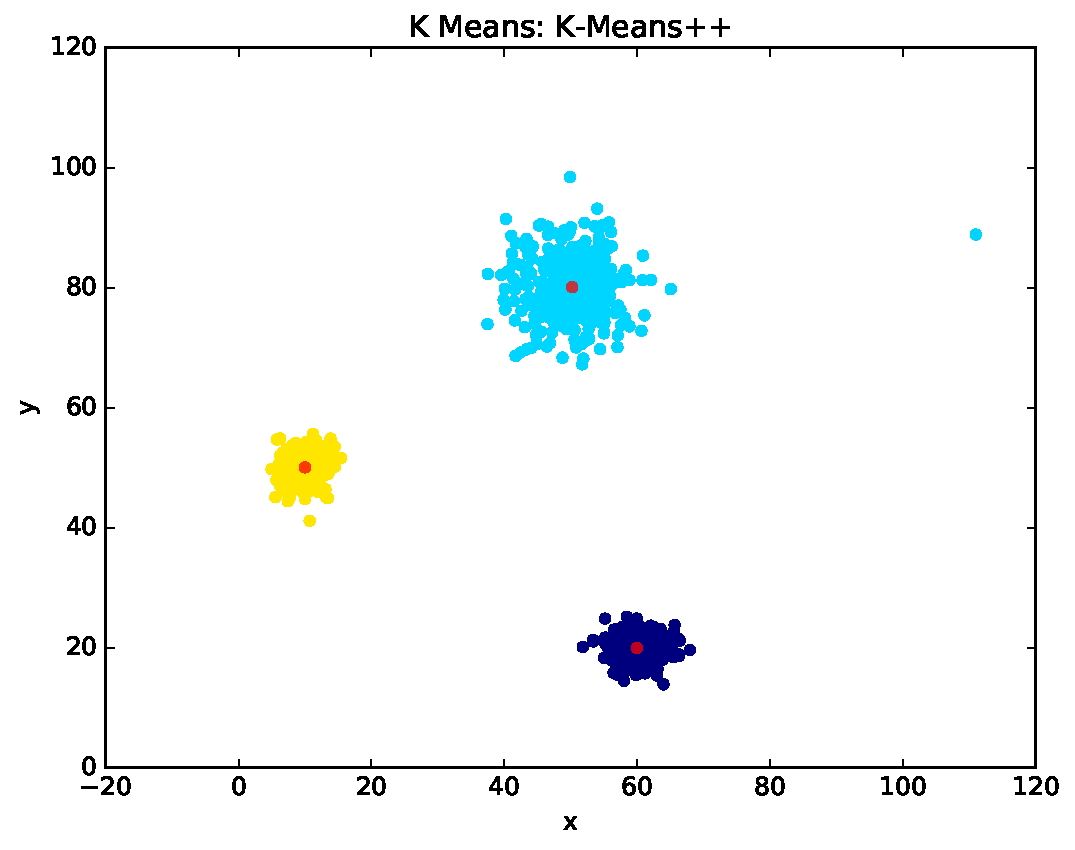
\includegraphics[width=.75\textwidth]{kmeanspp.pdf}
\caption{Clustering results with {\tt K-Means++}}
\end{figure}



\begin{table}[H]
\centering
\caption{Gonzalez Centroids}
\begin{tabular}{c c c}
\hline\hline
$c_{1}$ & $c_{2}$ & $c_{3}$\\
\hline
$(11.797, 49.467)$ & $(110.981, 88.871)$ & $(67.941, 19.630)$\\
\hline
\end{tabular}
\end{table}



\begin{table}[H]
\centering
\caption{$3$-Center Cost (Gonzalez)}
\begin{tabular}{c c c}
\hline\hline
$c_{1}$ & $c_{2}$ & $c_{3}$\\
$106.725$ & $114.176$ & $81.528$\\
\hline
\end{tabular}
\end{table}

\begin{table}[H]
\centering
\caption{$3$-Mean Cost (Gonzalez)}
\begin{tabular}{c c c}
\hline\hline
$c_{1}$ & $c_{2}$ & $c_{3}$\\
$1889.118$ & $7749.613$ & $2737.042$\\
\hline
\end{tabular}
\end{table}

\begin{figure}[H]
\centering
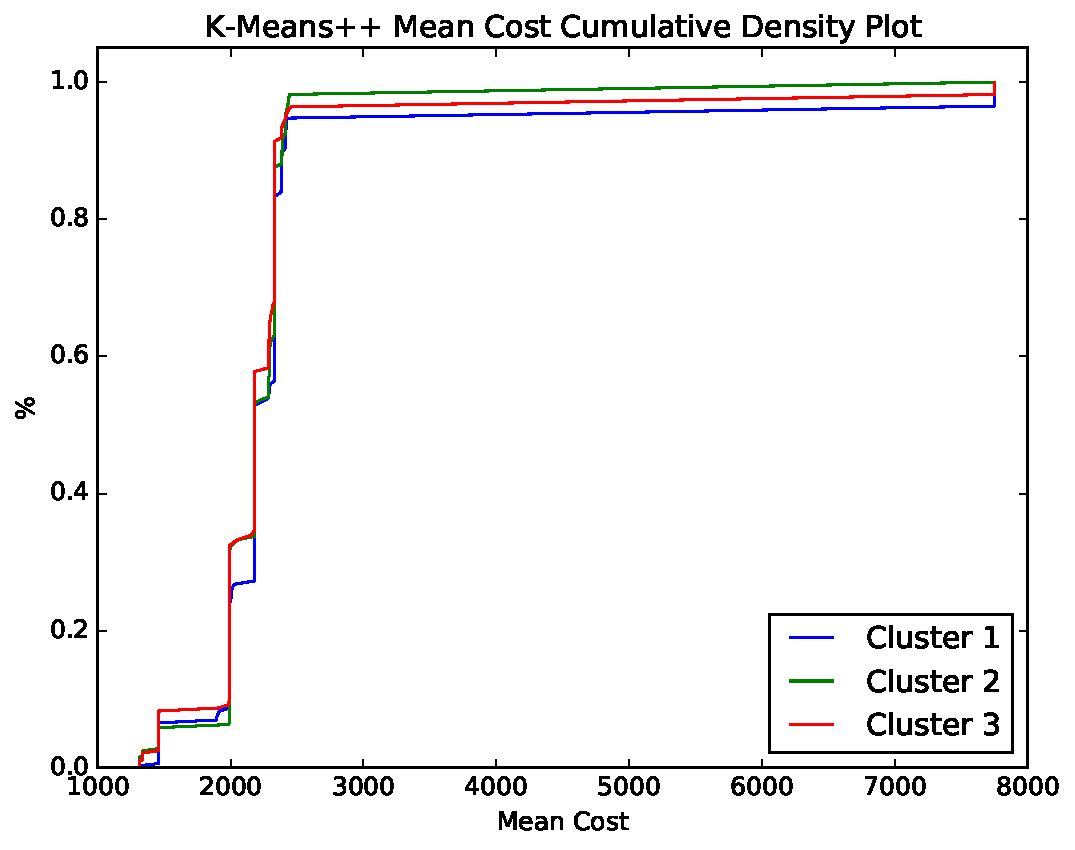
\includegraphics[width=.75\textwidth]{cdf.pdf}
\caption{ $3$-Mean Cost of {\tt K-Means++}}
\end{figure}

\paragraph{B: (20 points)}
Recall that Lloyd's algorithm for $k$-means clustering starts with a set of $k$ centers $C$ and runs as described in Algorithm 10.1.1.  

\begin{itemize}
\item  Run Lloyds Algorithm with $C$ initially with points indexed $\{\texttt{1,2,3}\}$.  Report the final subset and the $3$-means cost.  
\item  Run Lloyds Algorithm with $C$ initially as the output of \textsf{Gonzalez} above.  Report the final subset and the $3$-means cost.  
\item  Run Lloyds Algorithm with $C$ initially as the output of each run of \textsf{k-Means++} above.  Plot a \emph{cumulative density function} of the $3$-means cost.  Also report the fraction of the trials that the subsets are the same as the input (where the input is the result of \textsf{k-Means++}).  


\begin{figure}[H]
\centering
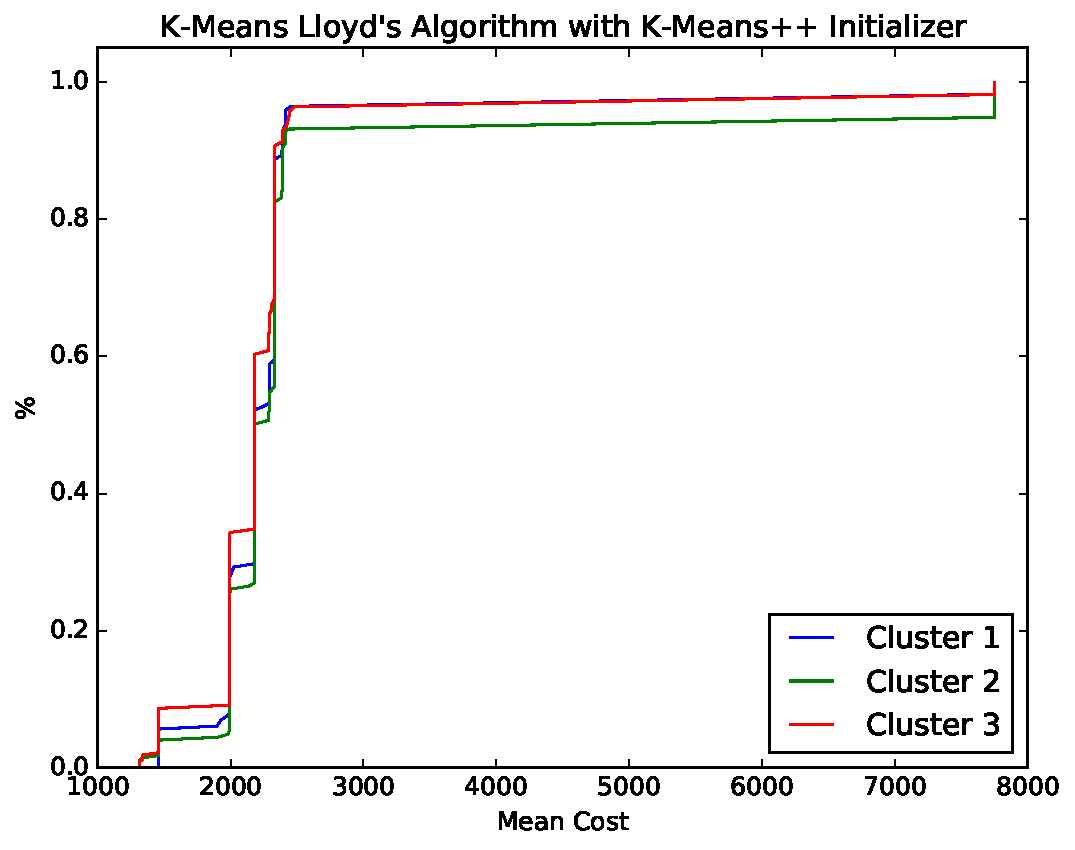
\includegraphics[width=.75\textwidth]{kmeanspp_lloyds.pdf}
\caption{$3$-Means cost for Lloyd's}
\end{figure}
\end{itemize}

%
%\paragraph{C: (10 points)}
%Consider a set of points $S \subset \bb{R}^d$ and $\D$ the Euclidean distance.  
%Prove that 
%\[
%\arg \min_{p \in \bb{R}^d} \sum_{x \in S} (\D(x, p))^2 = \frac{1}{|S|} \sum_{x \in S} x.
%\]  
%
%
%\emph{
%Here are some suggested steps to follow towards the proof (note there are also other valid ways to prove this, but, for instance, achieving some of these steps will get you partial credit):
%\begin{enumerate} \denselist
%\item First prove the same results for $S \in \bb{R}^1$.  
%\subitem (a) Expand each term $(\D(x,p))^2 = (x-p)^2 = x^2 + p^2 - 2xp$.
%\subitem (b) Take the derivative of each term.
%\subitem (c) Add the above terms back together and find where the total derivative is 0.
%\item Show the results for each dimension can be solved independently (use properties of edge lengths in a right triangle -- you may want to just redo the above steps using vector calculus).  
%\end{enumerate}
%}
%

%%%%%%%%%%%%%%%%%%%%%%%%%%%%%%%%%%%%%%%%%%%%%%%%%%%%
%%%%%%%%%%%%%%%%%%%%%%%%%%%%%%%%%%%%%%%%%%%%%%%%%%%%
%%%%%%%%%%%%%%%%%%%%%%%%%%%%%%%%%%%%%%%%%%%%%%%%%%%%
\section{High-dimensional Distances (15 points)}
In class, we compared the volume of an $\ell_2$ ball centered at the origin, with the smallest box containing that ball.   Here I will ask you to calculate how much we will have to expand the radius of the ball to have the same volume as the box.  

Recall, the volume of a $d$-dimensional $\ell_2$ ball with radius $r$ is
\[
\mathsf{vol}(B(d,r)) = \frac{\pi^{d/2}}{\Gamma(d/2+1)} r^d.
\]
Here $\Gamma(z) = \int_{x = 0}^\infty x^{z-1} e^{-x} dx$ is known as the Gamma function.  It is known that $\Gamma(2) = 1$, $\Gamma(2.5) \approx 1.33$, $\Gamma(3) = 2$ and in general for integers $z$ that $\Gamma(z) = (z-1)!$ \emph{(that is a factorial, not just excitement)}.  

For any ball $B(d,r)$ (for instance one or radius $r=1$), let $\mathsf{vol(box}(d,r)) = (2r)^d$ be the volume of the smallest enclosing box.  Determine the value of $r' = c r$ (an expanded radius greater than $r$) that we would have to expand the ball to so that it is the same as $\mathsf{vol(box}(d,r))$.  
Solve for the expansion factor $c$:
\begin{enumerate}
\item for $d=2$

{\tt 1.128}

\item for $d=3$

{\tt 1.241}


\item for $d=4$, and

{\tt 1.342}

\item as a function of $d$ (for large $d$), restricting to even values of $d$.

\[
  c = \left( \frac{\left[2^{-d}r^{d}\frac{\pi^{d/2}}{\Gamma (d/2 + 1)}\right]}{r} \right)^{-1}
\]
  
\item Plot the expansion factor $c$ up to $d=20$.  


\begin{figure}[H]
\centering
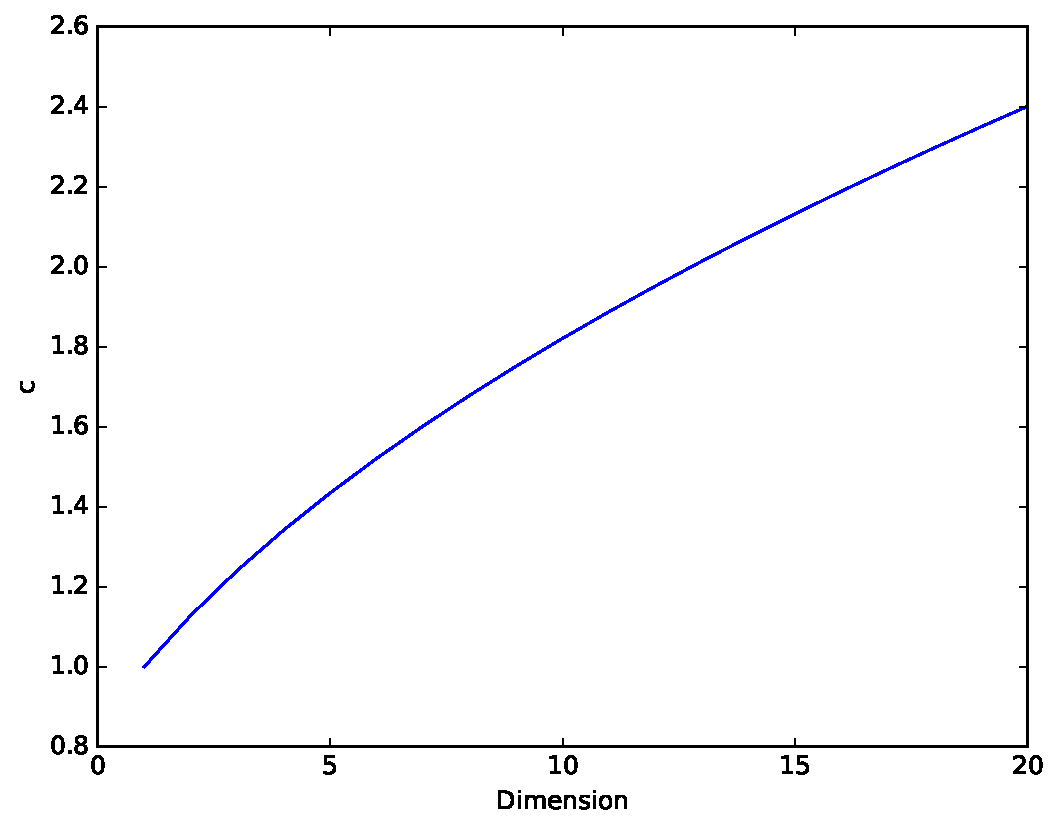
\includegraphics[width=.75\textwidth]{high_dimension.pdf}
\end{figure}

\end{enumerate}



%%%%%%%%%%%%%%%%%%%%%%%%%%%%%%%%%%%%%%%%%%%%%%%%%%%%
%%%%%%%%%%%%%%%%%%%%%%%%%%%%%%%%%%%%%%%%%%%%%%%%%%%%
%%%%%%%%%%%%%%%%%%%%%%%%%%%%%%%%%%%%%%%%%%%%%%%%%%%%
\section{$k$-Median Clustering (25 points)}
The $k$-median clustering problem on a data set $P$ is to find a set of $k$-centers $C = \{c_1, c_2, \ldots, c_k\}$ to minimize
$
\textsf{Cost}_1(P,C) = \frac{1}{|P|}\sum_{p \in P} \D(p, \phi_C(p)).
$
We did not explicitly talk much about this formulation in class, but the techniques to solve it are all typically extensions of approaches we did talk about.  This problem will be more open-ended, and will ask you to try various approaches to solve this problem.  We will use data set \texttt{C3.txt}.  


\paragraph{A: (20 points)}
Find a set of $4$ centers $C = \{c_1, c_2, c_3, c_4\}$ for the $4$-medians problem on dataset \texttt{C3.txt}.  Report the set of centers, as well as $\textsf{Cost}_1(P,C)$.  The centers should be in the write-up you turn in, but also in a file formatted the same was as the input so we can verify the cost you found.  That is each line has 1 center with 6 tab separated numbers.  The first being the index (e.g., 1, 2, 3 or 4), and the next 5 being the $5$-dimensional coordinates of that center.  

Your score will be based on how small a $\textsf{Cost}_1(P,C)$ you can find.   You can get 15 points for reasonable solution.  The smallest found score in the class will get all 20 points.  Other scores will obtain points in between.  

Very briefly describe how you found the centers.  


\begin{table}[H]
\centering
\caption{Centroids for $\left| C \right| = 4$}
\begin{tabular}{c | r r r r r}
\hline\hline
 & $x_{1}$ & $x_{2}$ & $x_{3}$ & $x_{4}$ & $x_{5}$\\
$c_{1}$ & $0.188$ & $0.845$ & $0.141$ & $0.132$ & $0.037$\\
$c_{2}$ & $1.007$ & $0.120$ & $-0.164$ & $0.085$ & $0.190$\\
$c_{3}$ & $-0.035$ & $0.106$ & $0.945$ & $0.044$ & $-0.134$\\
$c_{4}$ & $-0.257$ & $0.766$ & $0.209$ & $0.191$ & $0.141$\\
\hline
\end{tabular}
\end{table}

\begin{table}[H]
\centering
\caption{Mean Cost for $\left| C \right| = 4$}
\begin{tabular}{c c c c}
\hline\hline
$c_{1}$ & $c_{2}$ & $c_{3}$ & $c_{4}$\\
\hline
$0.303$ & $0.238$ & $0.411$ & $0.220$\\
\hline
\end{tabular}
\end{table}

\begin{figure}[H]
\centering
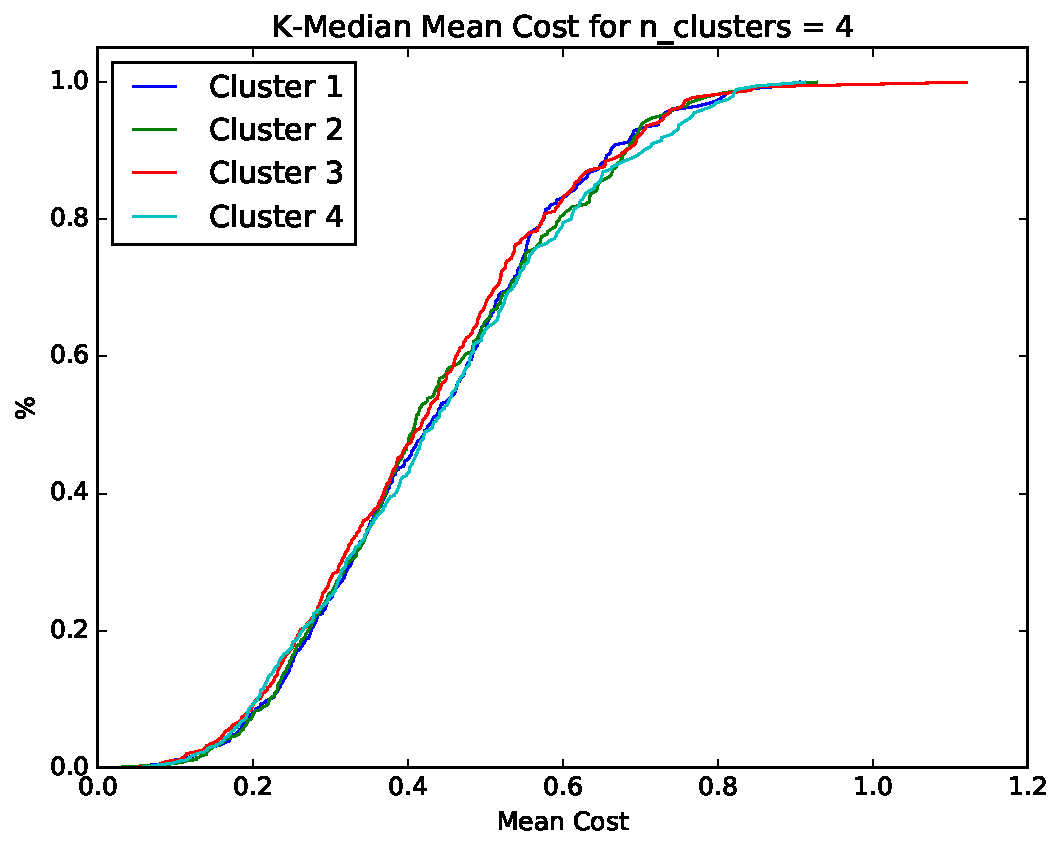
\includegraphics[width=.75\textwidth]{cdf_median_n-4.pdf}
\end{figure}



\paragraph{B: (5 points)}
Run your algorithm again for the $5$-medians problem on dataset \texttt{C3.txt}.  Report the set of $5$ centers and the $\textsf{Cost}_1(P,C)$.  You do not need to turn in a file for these, just write it in your report.  

\begin{table}[H]
\centering
\caption{Centroids for $\left| C \right| = 5$}
\begin{tabular}{c | r r r r r}
\hline\hline
 & $x_{1}$ & $x_{2}$ & $x_{3}$ & $x_{4}$ & $x_{5}$\\
$c_{1}$ & $-0.016$ & $0.075$ & $1.180$ & $-0.050$ & $-0.113$\\
$c_{2}$ & $0.008$ & $-0.096$ & $0.633$ & $0.135$ & $0.034$\\
$c_{3}$ & $-0.087$ & $-0.306$ & $0.053$ & $0.848$ & $0.222$\\
$c_{4}$ & $-0.025$ & $0.187$ & $0.115$ & $0.218$ & $0.686$\\
$c_{5}$ & $0.077$ & $-0.147$ & $0.743$ & $-0.087$ & $0.093$\\
\hline
\end{tabular}
\end{table}


\begin{table}[H]
\centering
\caption{Mean Cost for $\left| C \right| = 5$}
\begin{tabular}{c c c c c}
\hline\hline
$c_{1}$ & $c_{2}$ & $c_{3}$ & $c_{4}$ & $c_{5}$\\
\hline
$0.206$ & $0.243$ & $0.129$ & $0.328$ & $0.345$\\
\hline
\end{tabular}
\end{table}

\begin{figure}[H]
\centering
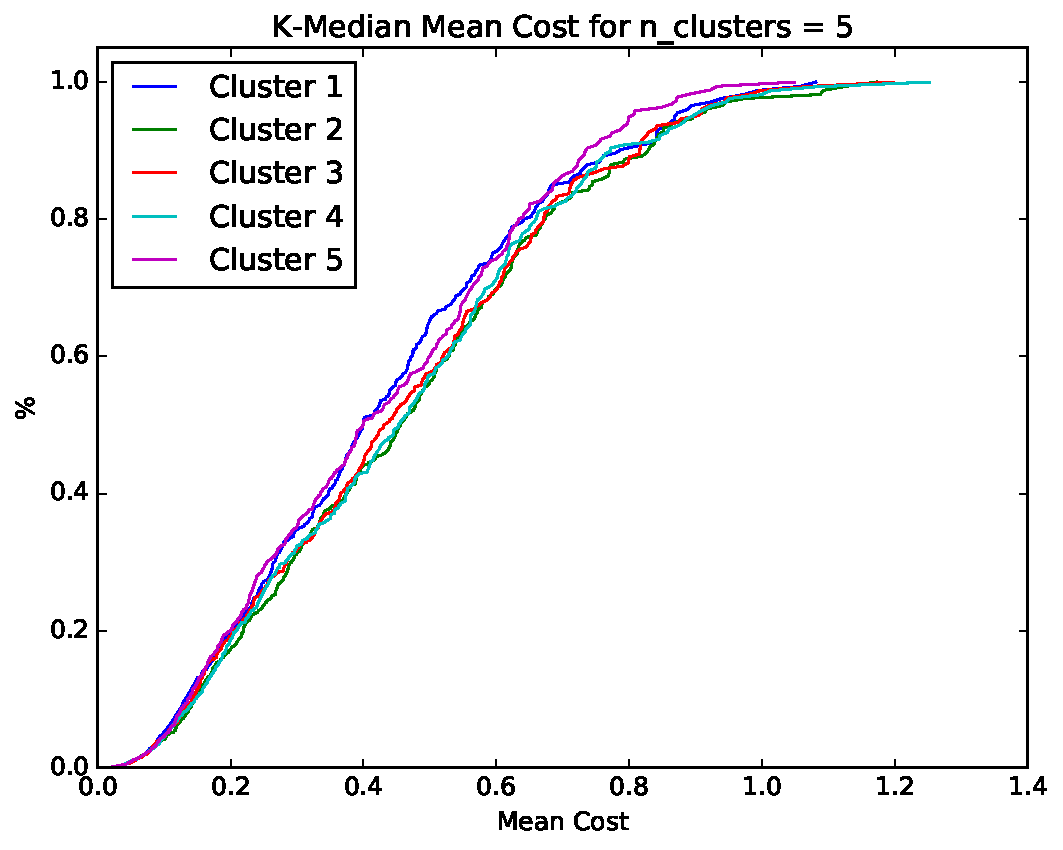
\includegraphics[width=.75\textwidth]{cdf_median_n-5.pdf}
\end{figure}



%%%%%%%%%%%%%%%%%%%%%%%%%%%%%%%%%%%%%%%%%%%%%%%%%%%%
%%%%%%%%%%%%%%%%%%%%%%%%%%%%%%%%%%%%%%%%%%%%%%%%%%%%
%%%%%%%%%%%%%%%%%%%%%%%%%%%%%%%%%%%%%%%%%%%%%%%%%%%%
%\section{BONUS (2 points)}

%Recall that the $k$-center problem is to find a set of $k$ centers $C$ to minimize
%\[
%\textsf{Cost}_0(P,C) = \max_{p \in P} \min_{c \in C} \D(p, c).
%\]

%Let $C^*$ be the optimal choice of $k$ centers for the $k$-center problem, and let $V^* = \textsf{Cost}_0(P,C^*)$.  

%Prove that the \textsf{Gonzalez} algorithm always finds a set of $k$ centers $C$ such that 
%\[
%\textsf{Cost}_0(P,C) \leq 2 V^*.
%\]





\end{document}
